\chapter*{Dodatak: Prikaz aktivnosti grupe}
		\addcontentsline{toc}{chapter}{Dodatak: Prikaz aktivnosti grupe}
		
		\section*{Dnevnik sastajanja}
		
		\textbf{\textit{Kontinuirano osvježavanje}}\\
		
		
		\begin{packed_enum}
				\item  sastanak
			
			\item[] \begin{packed_item}
				\item Datum: 14.10.2021.
				\item Prisustvovali: M.Barbir, M.Ivić, F.Bura, M.Žura, M.Puharić, L.Gjurić, Z.Ravlić
				\item Teme sastanka:
				\begin{packed_item}
					\item  Prvi sastanak tima
					\item  Formiranje grupe
				\end{packed_item}
			\end{packed_item}
			\item  sastanak
		
		\item[] \begin{packed_item}
			\item Datum: 26.10.2021.
			\item Prisustvovali: M.Barbir, M.Ivić, F.Bura, M.Žura, M.Puharić, L.Gjurić, Z.Ravlić
			\item Teme sastanka:
			\begin{packed_item}
				\item  Raspodjela na frontend i backend
				\item  Raspodjela rada na dokumentaciji
			\end{packed_item}
		\end{packed_item}
			\item  sastanak
			
			\item[] \begin{packed_item}
				\item Datum: 2.11.2021.
				\item Prisustvovali: M.Barbir, M.Ivić, F.Bura, M.Žura, M.Puharić, L.Gjurić, Z.Ravlić
				\item Teme sastanka:
				\begin{packed_item}
					\item  Rasprava o stanju na projektu
				\end{packed_item}
			\end{packed_item}
			
			\item  sastanak
			\item[] \begin{packed_item}
				\item Datum: 15.11.2021.
				\item Prisustvovali: M.Barbir, M.Ivić, F.Bura, M.Žura, M.Puharić, L.Gjurić, Z.Ravlić
				\item Teme sastanka:
				\begin{packed_item}
					\item  Rasprava o stanju na projektu
					\item  Pregled dokumentacije
					\item  Dogovor o deployju aplikacije 
				\end{packed_item}
			\end{packed_item}
		
			\item  sastanak
			\item[] \begin{packed_item}
				\item Datum: 3.12.2021.
				\item Prisustvovali: M.Barbir, M.Ivić, F.Bura, M.Žura, M.Puharić, L.Gjurić, Z.Ravlić
				\item Teme sastanka:
				\begin{packed_item}
					\item  Rasprava o stanju na projektu
					\item  Raspodijela poslova
					\item  Dogovor o razvoju alfa verzije 
				\end{packed_item}
			\end{packed_item}
		\item  sastanak
		\item[] \begin{packed_item}
			\item Datum: 13.12.2021.
			\item Prisustvovali: M.Barbir, M.Ivić, F.Bura, M.Žura, M.Puharić, L.Gjurić, Z.Ravlić
			\item Teme sastanka:
			\begin{packed_item}
				\item  Rasprava o stanju na projektu
				\item Rjesavanje problema na projektu
			\end{packed_item}
		\end{packed_item}
	\item  sastanak
	\item[] \begin{packed_item}
		\item Datum: 4.1.2022.
		\item Prisustvovali: M.Barbir, M.Ivić, F.Bura, M.Žura, M.Puharić, L.Gjurić, Z.Ravlić
		\item Teme sastanka:
		\begin{packed_item}
			\item  Rasprava o stanju na projektu
			\item  Pregled dokumentacije
			\item  Dogovor o razvoju zavrsne verzije aplikacije
		\end{packed_item}
	\end{packed_item}
\item  sastanak
\item[] \begin{packed_item}
	\item Datum: 14.1.2022.
	\item Prisustvovali: M.Barbir, M.Ivić, F.Bura, M.Žura, M.Puharić, L.Gjurić, Z.Ravlić
	\item Teme sastanka:
	\begin{packed_item}
		\item  Rasprava o stanju na projektu
		\item  Pregled dokumentacije
		\item  Dogovor o deploju aplikacije 
		\item  Rjesavanje problema
	\end{packed_item}
\end{packed_item}
			%
			
		\end{packed_enum}
		
		\eject
		\section*{Tablica aktivnosti}
		
			\textbf{\textit{Kontinuirano osvježavanje}}\\
			

			\begin{longtblr}[
					label=none,
				]{
					vlines,hlines,
					width = \textwidth,
					colspec={X[7, l]X[1, c]X[1, c]X[1, c]X[1, c]X[1, c]X[1, c]X[1, c]}, 
					vline{1} = {1}{text=\clap{}},
					hline{1} = {1}{text=\clap{}},
					rowhead = 1,
				} 
				\multicolumn{1}{c|}{} & \multicolumn{1}{c|}{\rotatebox{90}{\textbf{Marko Barbir}}} & \multicolumn{1}{c|}{\rotatebox{90}{\textbf{Luka Gjurić }}} &	\multicolumn{1}{c|}{\rotatebox{90}{\textbf{Marko Žura }}} & \multicolumn{1}{c|}{\rotatebox{90}{\textbf{Filip Bura }}} &	\multicolumn{1}{c|}{\rotatebox{90}{\textbf{Marin Puharić }}} & \multicolumn{1}{c|}{\rotatebox{90}{\textbf{Zvonimir Ravlić }}} &	\multicolumn{1}{c|}{\rotatebox{90}{\textbf{Mate Ivić }}} \\  
				
				Upravljanje projektom 		&10  &5  &5  &5  &9  &7  &2 \\ 
				Opis projektnog zadatka 	&0  &0  &12  &0  &0  &0  &0 \\ 
				
				Funkcionalni zahtjevi       &2  &0  &0  &0  &4  &0  &0  \\ 
				Opis pojedinih obrazaca 	&1  &0  &0  &4  &1.5  &5  &4  \\ 
				Dijagram obrazaca 			&0  &0  &0  &0  &0  &15  &10  \\ 
				Sekvencijski dijagrami 		&0  &0  &0  &0  &0  &0  &7  \\ 
				Opis ostalih zahtjeva 		&0  &0  &4  &0  &0  &0  &0  \\ 

				Arhitektura i dizajn sustava	 &0.5  &1  &1  &1  &0.5  &5  &1  \\ 
				Baza podataka				&2  &0  &0  &0  &0  &9  &0   \\ 
				Dijagram razreda 			&0  &0  &0  &0  &0  &10  &11   \\ 
				Dijagram stanja				&0  &0  &0  &0  &0  &5  &0  \\ 
				Dijagram aktivnosti 		&0  &0  &0  &0  &0  &5  &0  \\ 
				Dijagram komponenti			&0  &0  &0  &0  &0  &5  &0  \\ 
				Korištene tehnologije i alati 		&5  &0  &0  &5  &0  &0  &0  \\ 
				Ispitivanje programskog rješenja 	&7  &0  &0  &0  &10  &10  &0  \\ 
				Dijagram razmještaja			&0  &0  &0  &0  &0  &3  &0  \\ 
				Upute za puštanje u pogon 		&0  &0  &0  &0  &0  &3  &0  \\  
				Dnevnik sastajanja 			&2  &1  &1  &0.5  &0.5  &1  &1  \\ 
				Zaključak i budući rad 		&0  &0  &0  &0  &0  &0.5  &0  \\  
				Popis literature 			&0  &0  &0  &0  &0  &0  &0  \\  \hline 
				
				Izrada početne stranice 			&10  &15  &1  &0  &10  &0  &2  \\  
				Izrada baze podataka	 			&5  &0  &0  &0  &0  &3  &0 \\  
				Spajanje s bazom podataka 			&4  &2  &0  &5  &4  &0  &0  \\ 
				Back end 							&150  &25  &25  &40  &130  &40  &50  \\  
				Front end							&60  &90  &30  &20  &30  &35  &20\\
				Deployment na Heroku				&10  &0  &0  &15  &5  &0  &0
			\end{longtblr}
					
					
		\eject
		\section*{Dijagrami pregleda promjena}
		
			\begin{figure}[H]
			
			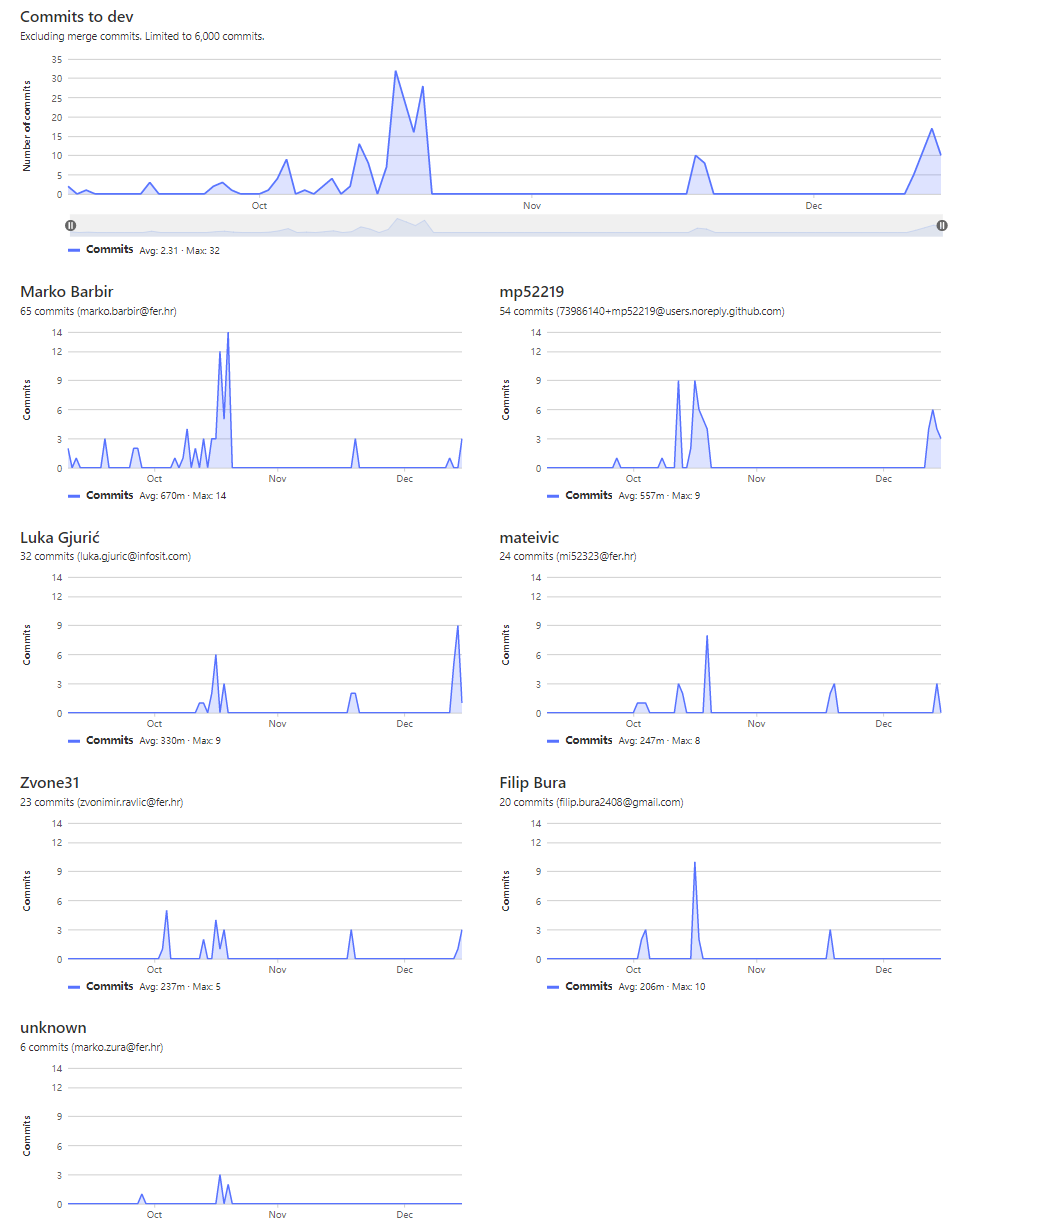
\includegraphics[width=\textwidth]{slike/commits.png} %veličina slike u odnosu na originalnu datoteku i pozicija slike
			\centering
			\caption{Commits}
			\label{fig:commits}
		\end{figure}
	